% -*- Mode: TeX -*-
% for LaTeX
\documentclass{slides}
\usepackage{epsfig}

\def\slidetitlenocoin#1{\begin{center}\large #1 \end{center}}
\def\tinytiberius{\raisebox{-.1in}{\mbox{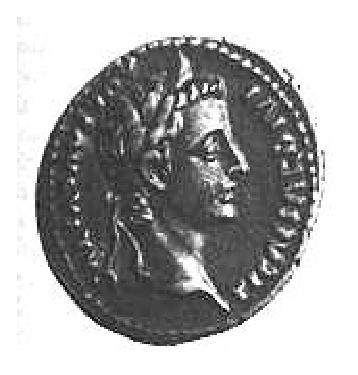
\epsfig{file=tiberius-coin.eps,height=.5in}}}}
\def\tinycaligula{\raisebox{-.1in}{\mbox{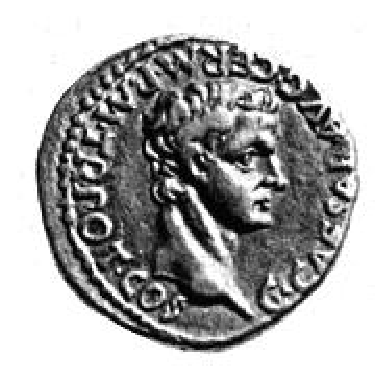
\epsfig{file=caligula-coin.eps,height=.5in}}}}
\def\slidetitle#1{\begin{center}\tinytiberius \hfill {\large #1} \hfill
    \tinycaligula \end{center} \vspace{-.4in} \strut\hrulefill\strut}
% 1in doesn't seem to work.  Perhaps need to put caption *after* slide, to
% overwrite it.
% \def\raisedslidetitle#1{\centerline{\raisebox{1.5in}[2ex]{{\large #1}}}
% \def\raisedslidetitle#1{\centerline{\raisebox{1in}[2ex]{\large #1}}}
\def\raisedslidetitle#1{\centerline{\raisebox{.5in}[2ex]{\makebox[\textwidth]{\tinytiberius \hfill {\large #1} \hfill \tinycaligula}}}}
% With 6.5in or 7in, text ran off page
\def\epsheight{6in}
\def\slbreak{\\ \strut\hspace{1em}}

\makeatletter
\def\nopgbrk{\@nobreaktrue}
\makeatother

\begin{document}
\partopsep 0pt
\topsep 0pt

\begin{slide}
\slidetitlenocoin{\mbox{\hspace{-36pt}An Empirical Analysis of C Preprocessor Use}}
\vspace{.3in}
\centerline{Michael Ernst}
\vspace{.3in}
\centerline{joint work with Greg Badros and David Notkin}

% Efforts to smooth these, turn them into gifs and edit out the noise,
% etc., produced much worse results than the plain PostScript files.
  $$
  \begin{array}{c}
    \mbox{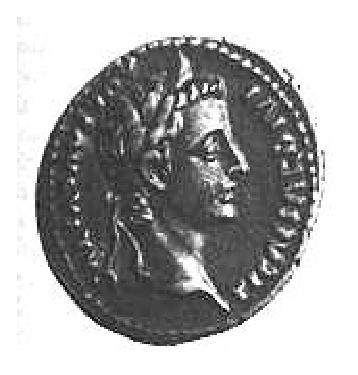
\epsfig{file=tiberius-coin.eps,height=2.75in}}
  \end{array}
  \mbox{~~~~~}
  \begin{array}{c}
    \mbox{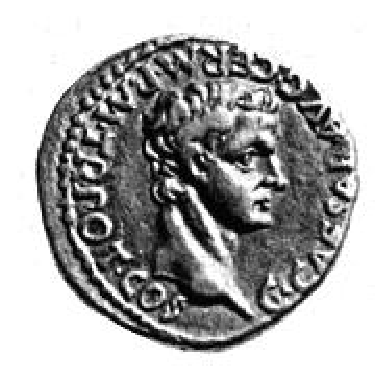
\epsfig{file=caligula-coin.eps,height=2.75in}}
  \end{array}
  $$

\end{slide}

\begin{note}
Please interrupt to ask questions.

Goal: better understand how the preprocessor is used.  (It can be used in a
disciplined, limited way to reduce programmer effort and improve
readability, readability, and performance.   Or, it can almost obliterate
the code.  Which do people use in practice?)  (Answer: both; there is good
news and bad news, no matter what your goals.)

(Tiberius Caesar; his son and successor Gaius; 
Naevius Macro was head of his Praetorian Guard;
Tacitus states in the {\em Annals}, ``By AD 37, the influence of Macro was
supreme''; I think 1,960 years is long enough.)

\end{note}

\begin{slide}
\slidetitle{Who cares?}

Language designers

Tool writers

Programmers

Software engineers
\end{slide}

\begin{note}
Language designers: see what's missing, see what people do via macros and
Cpp, figure out how to support it (or prevent it!) \slbreak
Think more about this:  Also, how do language choices lead to more/less
tightly integrated (as opposed to open, component-based) environments?
E.G., no need for \verb|__LINE__| in Java?

Tool writers: understand how people use Cpp; learn to recognize and cope
with those constructs. \slbreak
Translator \& other macro tool writers:  Is this a reasonable task?  Is it a
non-trivial task?

Programmers: see how to avoid constructs that give tools fits.  Or, learn
weird new tricks!

Software engineers: This has never been done before -- try it and see
what's interesting.  This may seem straightforward, but we discovered some
interesting results; both good and bad news.  [Briefly mention (lack of)
related work here?]
\end{note}


\def\outlineslidebody{
  \slidetitle{Outline}

  Motivation

  Results
  \vspace{-.5in}
  \begin{itemize}\itemsep 0pt \parskip 0pt
  \item preprocessor usage
  \item macro definitions
  \item macro expansions
  \item macro categorization
  \end{itemize}

  Conclusions
}

\begin{slide}
\outlineslidebody
\end{slide}

\begin{note}

Motivation:  why do we care? \slbreak
Because Cpp is evil.

Results
\vspace{-.5in}
\begin{itemize}\itemsep 0pt \parskip 0pt
\item 1 million lines of publicly-available C source
\item preprocessor usage: percentages and breakdown
\item macro definitions: number of definitions, categorize bodies
\item macro expansions: number of expansions, where and how often expanded
\end{itemize}

\end{note}

\begin{slide}
\slidetitle{Cpp considered harmful}

Cpp is essential
\vspace{-.5in}
\begin{itemize}\itemsep 0pt \parskip 0pt
\item file inclusion
\item define constants and macros
\item conditional compilation
\end{itemize}

Cpp is hard to reason about
\end{slide}

\begin{note}
(Say ``C preprocessor'' on this slide.)

Macros are an extra-language feature without which C is incomplete: you
can't write a C program without Cpp.

Hard for both tools and people to reason about. \slbreak
A ``C program'' isn't really C, so existing tools don't help. \slbreak
Macros can expand to anything you want --- very arbitrary.
\end{note}

\begin{slide}
\slidetitle{Coping with Cpp}

Ignore it

Preprocess into Cpp-free C code
\vspace{-.5in}
\begin{itemize}\itemsep 0pt \parskip 0pt
\item program must parse
\item tool and human see different inputs
\item loss of information
\item one configuration, not whole program
\end{itemize}

Operate on un-preprocessed code
\end{slide}

\begin{note}
\vspace{-40pt} % To make this note fit on one page.
{\small
I'm talking about both humans and tools, but with an emphasis on tools.

Ignoring Cpp is acceptable (only) for approximate tools.

Problems with pre-processing:
\vspace{-.3in}
\begin{itemize}\itemsep 0pt \parskip 0pt
\item syntactic: what about porting, maintenance?
\item tool input is not what user sees; back mappings are imperfect (and
  some tools don't even try)
\item loss of information:
% \vspace{-.5in}
\begin{itemize}\itemsep 0pt \parskip 0pt
  \item {\tt \#define}s don't appear in symbol table
  \item less documentation (e.g., types on constants and functions)
  \item can't trace or break on macros; can do so for inline functions
\end{itemize}
\item can only reason about one specialization or configuration, not about
  the program as a whole
\end{itemize}

Operate on un-preprocessed code: \slbreak
ambitious and difficult, so we did this. \slbreak
(Complicated preprocessor use, complicated mappings between original and processed.)
}
\end{note}

\begin{slide}
\slidetitle{Coping with Cpp, continued}

Test for, perhaps annotate, tricky uses

Eliminate in favor of {\tt const}, {\tt inline}, templates, reference
parameters


\end{slide}

\begin{note}
Like macro lint.

Elimination does away all the problems listed above, because tools can
already deal with regular C code.  We can do this via a source-to-source
translation.  (This was my real motivation.)
\end{note}


\begin{slide}
\slidetitle{Cpp: not all bad}

Language extensions

No dependence on compiler

Some tools exist
\end{slide}

\begin{note}
Can define entirely new syntax, avoid repetition, do other things the
language doesn't let you do.  [more examples here!]

No compiler dependence:
\vspace{-.5in}
\begin{itemize}\itemsep 0pt \parskip 0pt
\item inlining (probably -- watch out for recursion, etc.)
\item constant-folding
\item fold away branches
\end{itemize}
Should trust the compiler more than the programmer most (not all) of the time

Tool examples: Emacs hide-ifdef mode

There are killer apps for Cpp: 
\vspace{-.5in}
\begin{itemize}\itemsep 0pt \parskip 0pt
 \item conditional compilation (esp. system dependencies)
 \item declarations (writing two different languages in one source code)
 \item repetitive constructs
\end{itemize}

\end{note}


\begin{slide}
\outlineslidebody
\end{slide}

\begin{note}
Empty note.
\end{note}


\begin{slide}
% \vspace{-1in}
% \slidetitle{Cpp use}
\raisedslidetitle{Cpp use}

\centerline{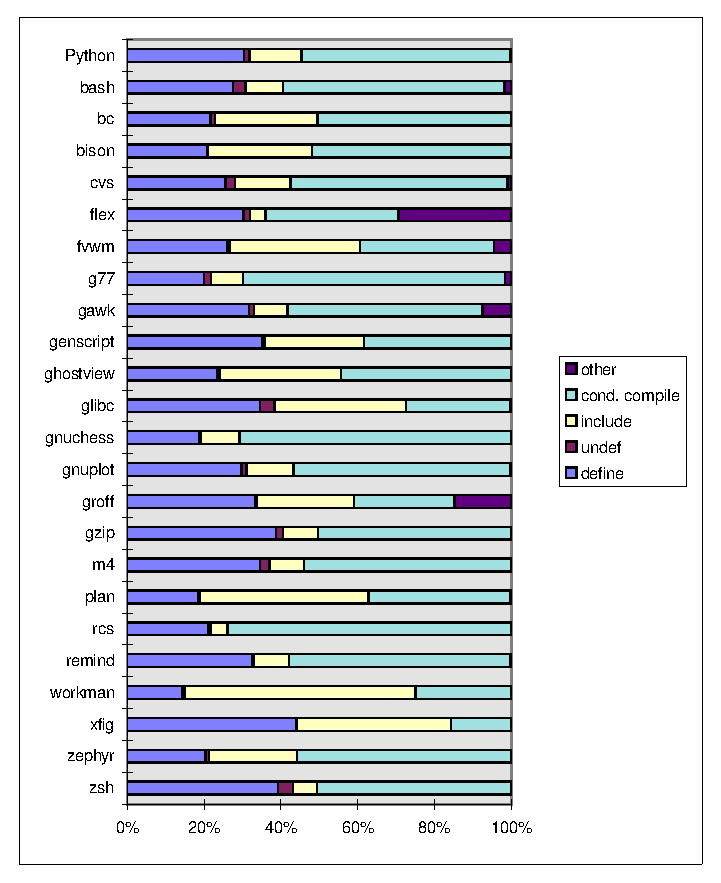
\epsfig{file=directives-breakdown.eps,height=\epsheight}}

Cpp: 10\% of non-comment non-blank lines
\end{slide}

\begin{note}
\small

Lots of Cpp use ($\frac{1}{9}$ more than 21\%)
% \vspace{-.5in}
\begin{itemize}\itemsep 0pt \parskip 0pt
 \item conditional compilation: 46\%
 \item macro definition: 31\%
 \item file inclusion: 19\%
 \item macro undefinition: 2\%
 \item that's all (duh)
\end{itemize}

Lots of variation

{\tt \#undef} almost always precedes a definition, to avoid warnings

{\tt \#line} appears only in lex and yacc output (for bootstrapping, or
when they aren't available)

Heavy Cpp users:
% \vspace{-.5in}
\begin{itemize}\itemsep 0pt \parskip 0pt
\item gzip: lots of {\tt \#define} for literals, system calls
\item glibc: lots of {\tt \#include}, many small files (avg.~42 lines);
  libraries are weird
\item remind: {\tt \#define} for all output,
  conditional compilation checks of \verb|HAVE_PROTO|
\item bash: many tests for availability of system services
\end{itemize}
\end{note}


% \begin{slide}
% % \slidetitle{Breakdown by package}
% % \slidetitle{Relative incidence of directives}
% \centerline{\raisebox{1in}[2ex]{\large Relative incidence of directives}}
% \nopgbrk
% % [7in] is too big, goes to next page
% \centerline{\raisebox{-1in}[6in][0pt]{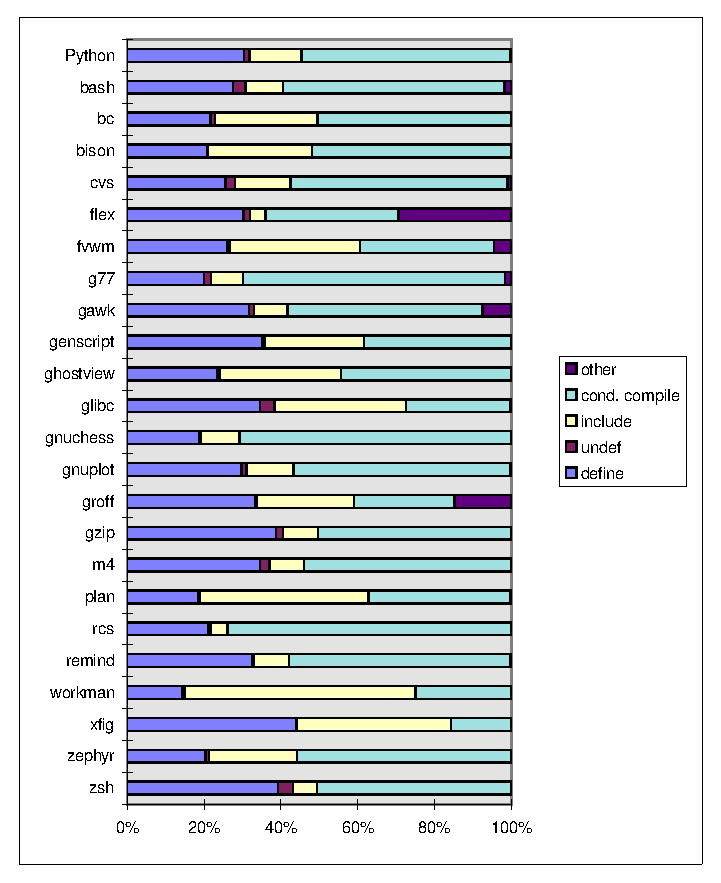
\epsfig{file=directives-breakdown.eps}}}
% \end{slide}
% 
% \begin{note}
% Lots of variation:
% \vspace{-.5in}
% \begin{itemize}\itemsep 0pt \parskip 0pt
% \item define: 14x
% \item conditional: 16x
% \item include: 25x
% \end{itemize}
% \end{note}


\begin{slide}
\raisedslidetitle{Definitions per Cpp identifier}

\centerline{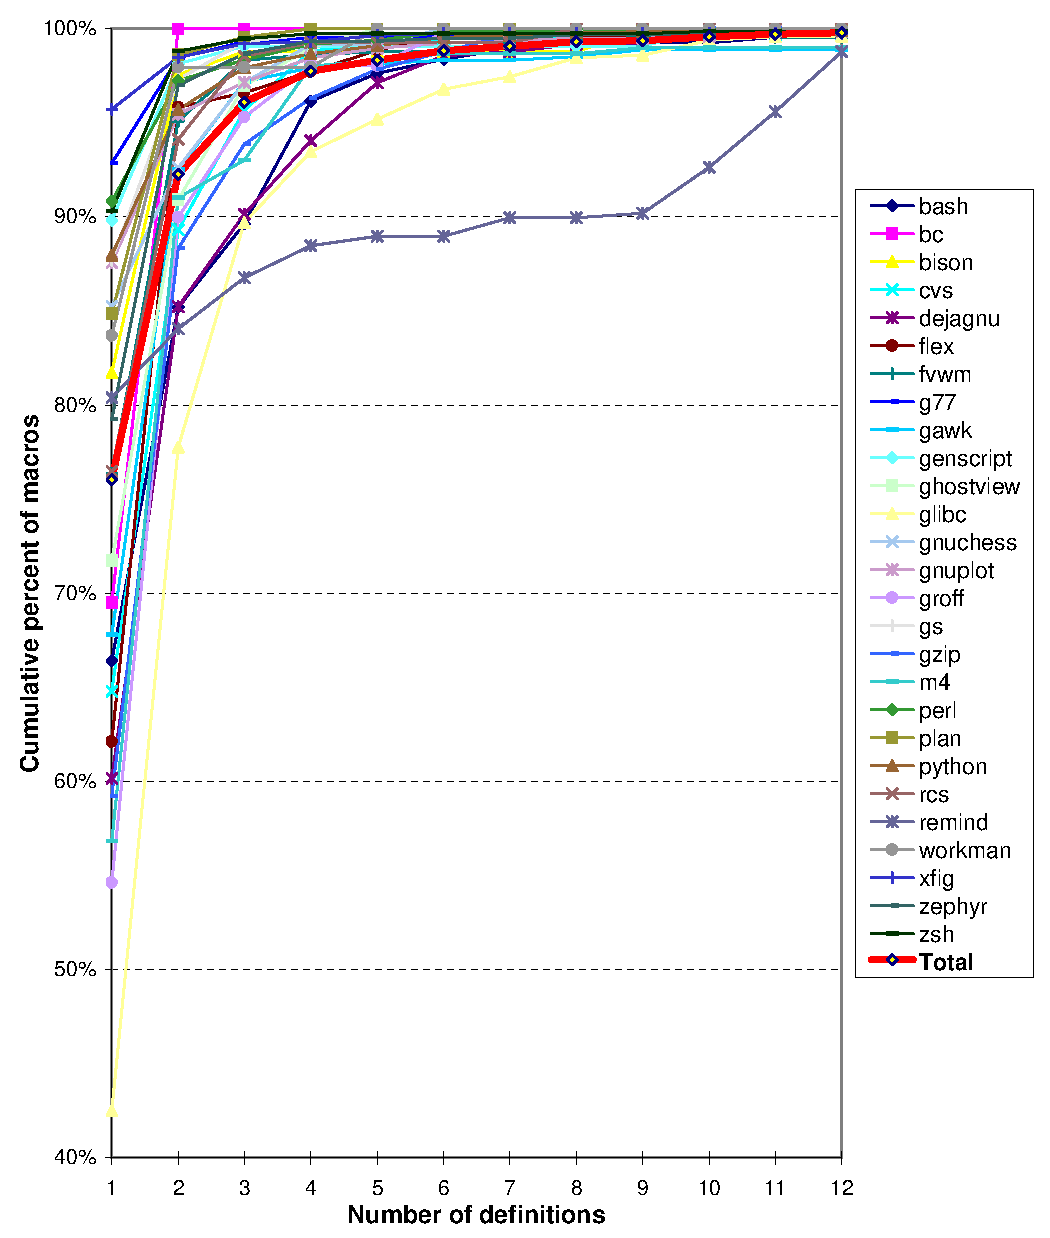
\epsfig{file=def-frequency.eps,height=\epsheight}}

24\% of macros are defined more than once

96\% of macros are defined three or fewer times
\end{slide}

\begin{note}
Surprising: so many definitions for so many macros.  But the tail is pretty
short.

Basically good news.

When multiple defs, they often (not always) have same type or same effect
on parser state.  (Maybe refer to a later analysis (categorization by macro
identifier rather than by macro definition), if I can do it in time.)

bc: all macros have 1 or 2 different expansions

remind: over 10\% of macros expand to more than 8 texts (all defined $\le
14$ times)

16 macros defined $> 16$ times; 3 defined $>30$ times.
\end{note}

\begin{slide}
\raisedslidetitle{Expansions per Cpp macro}

\centerline{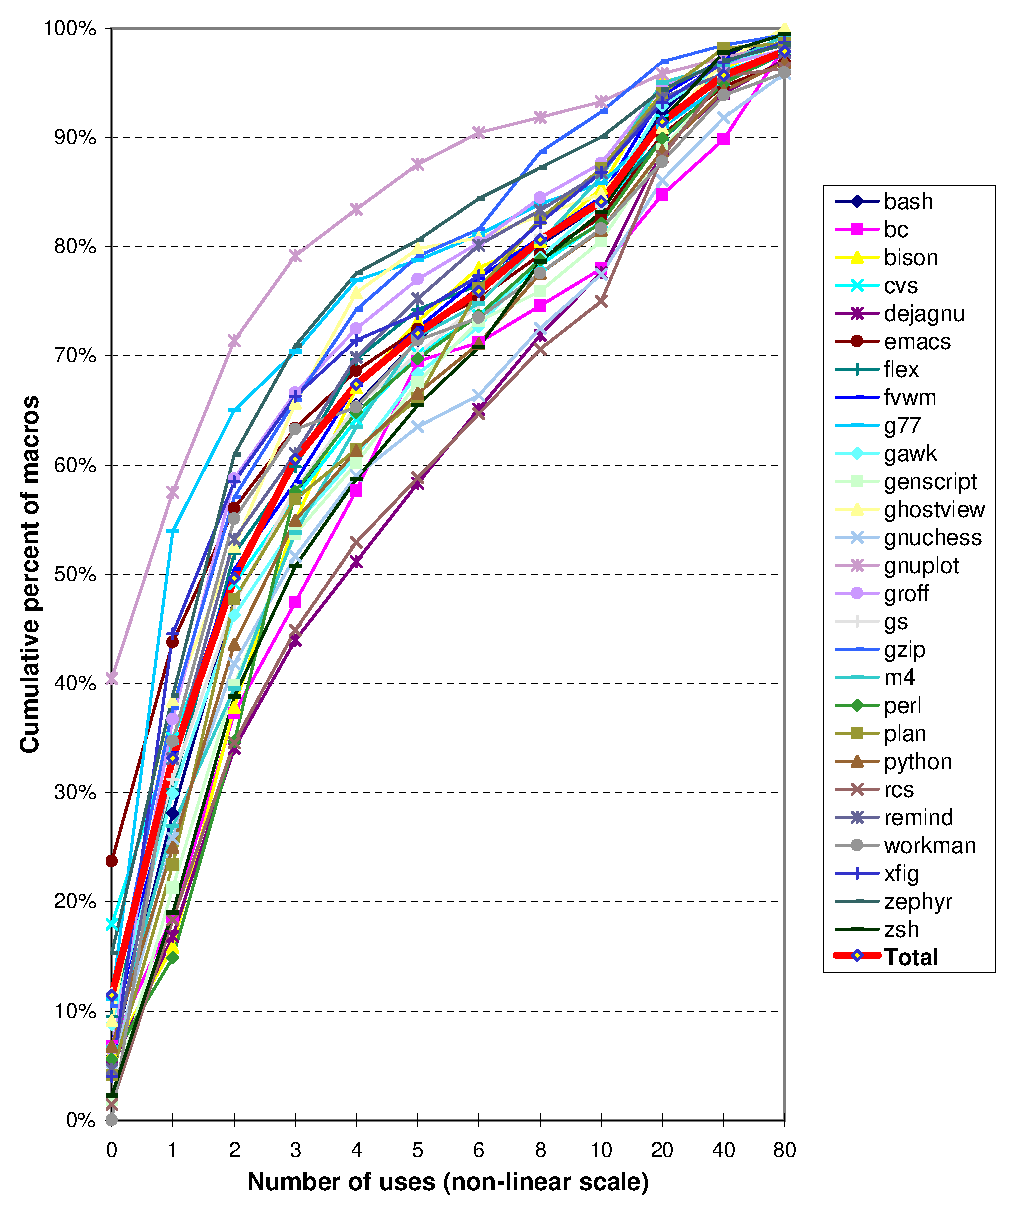
\epsfig{file=use-frequency.eps,height=\epsheight}}

82\% of macros are expanded 8 or fewer times

13\% of macros are never expanded
\end{slide}

\begin{note}
The interesting data are at the extrema:  pretty many not used, and tail is
very long.  Notice the scaling of the bottom axis (go to a log scale??)

unused percentage is usually between 4\% and 12\%; gnuplot very high

glibc is a library, so it isn't surprising that it defines many macros it
never uses itself -- they're intended for external consumption.

Tail of the distribution:
\begin{itemize}
  \item 99\%: 147 expansions
  \item 99.5\%: 273 expansions
  \item 99.9\%: 882 expansions
  \item python uses {\tt NULL} 4233 times
\end{itemize}
\end{note}

\begin{slide}
\raisedslidetitle{Where macros are used}

\centerline{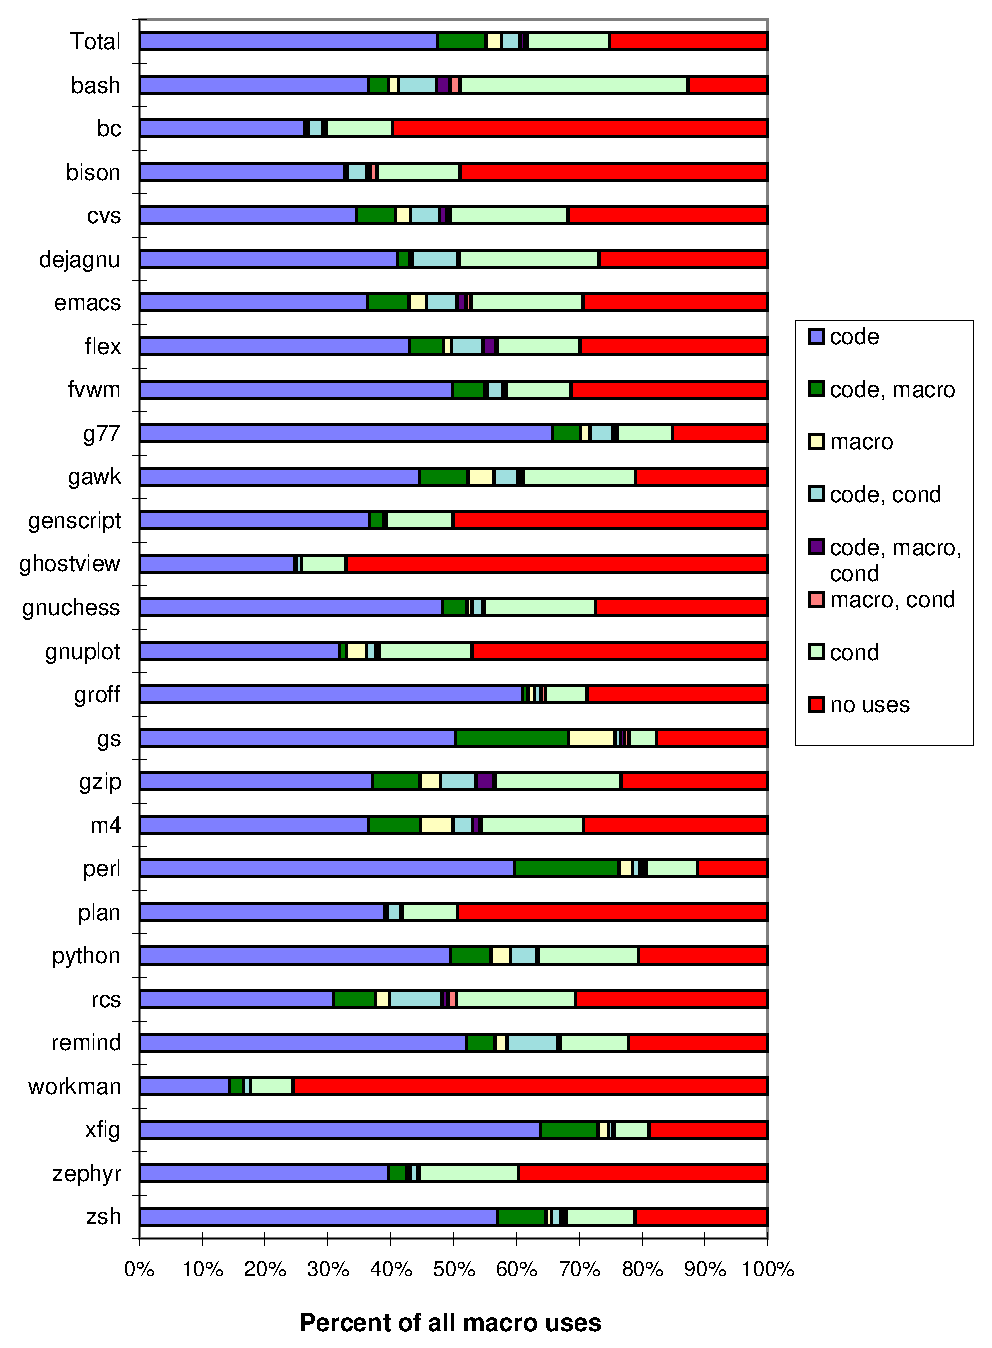
\epsfig{file=where-used.eps,height=\epsheight}}

3.1\% of macros appear in both code and conditional contexts

\end{slide}

\begin{note}
macro and conditional accounts for 0.2\%

conditional compilation accounts for half of Cpp directives but only 5.4\%
of macros (plus 3.1\% for macros also used by code)
\end{note}

\begin{slide}
\slidetitle{Categorization}

Null define: {\tt \#define \verb|HAVE_PROTO|}

Constant: {\tt \#define \verb|ARG_MAX| 131072} \slbreak
{\tt \#define \verb|RED_COLS| (1 << \verb|RED_BITS|)}

Expression: {\tt \#define sigmask(x) (1 << ((x)-1))}

Statement: {\tt \#define FREE(s) if (s) free(s);}

Stringization and pasting: \slbreak
  {\tt \#define \verb|__CONCAT|(x,y) x \#\# y}

Other syntactic macros: {\tt \#define AND ;} \slbreak
  {\tt \#define private static}

Type-related: {\tt \#define \verb|__ptr_t| void *} \slbreak
  {\tt \#define PTRBITS \verb|__BITS|(char*)}

Recursive: {\tt \#define LBIT vcat(LBIT)}

Failed classification: \slbreak
  {\tt \#define \verb|DO_OP|(OP,a,b) (a OP b)}
%  {\tt \#define \verb|SYSDEP_CFLAGS| -q \verb|no_sl_enable|}
\end{slide}

\begin{note}
\small
% \vspace{-1in}
This is the only place where previous work is at all applicable.
(Their categorizations sometimes focussed on constructs that don't happen
all that often or missed ones that are actually frequent.)

% \vspace{-.5in}
\begin{itemize}\itemsep 0pt \parskip 0pt
\item Null define: can be in Cpp or in code (get private = static or nothing)
\item Constant: includes literals
\item Expression: might be constant or might have different value.  Like a
function not returning void.
\item Statement: like a function returning void.
\item Stringization and pasting: uses arg as text
\item Other syntactic macros: e.g. private = static, partial declarations
\item Type-related: type as argument, pass a type, expand to a type, or use
  such a macro
\item Recursive: extend of previously-defined macros
\item Failed classification: more partial declarations (2\%; could go well
  below 1\% by doing single level of macro expansion, as one macro def \&
  uses accounts for 50\% of failures)
\end{itemize}

\end{note}

\begin{slide}
\raisedslidetitle{Macro body categorizations}

\centerline{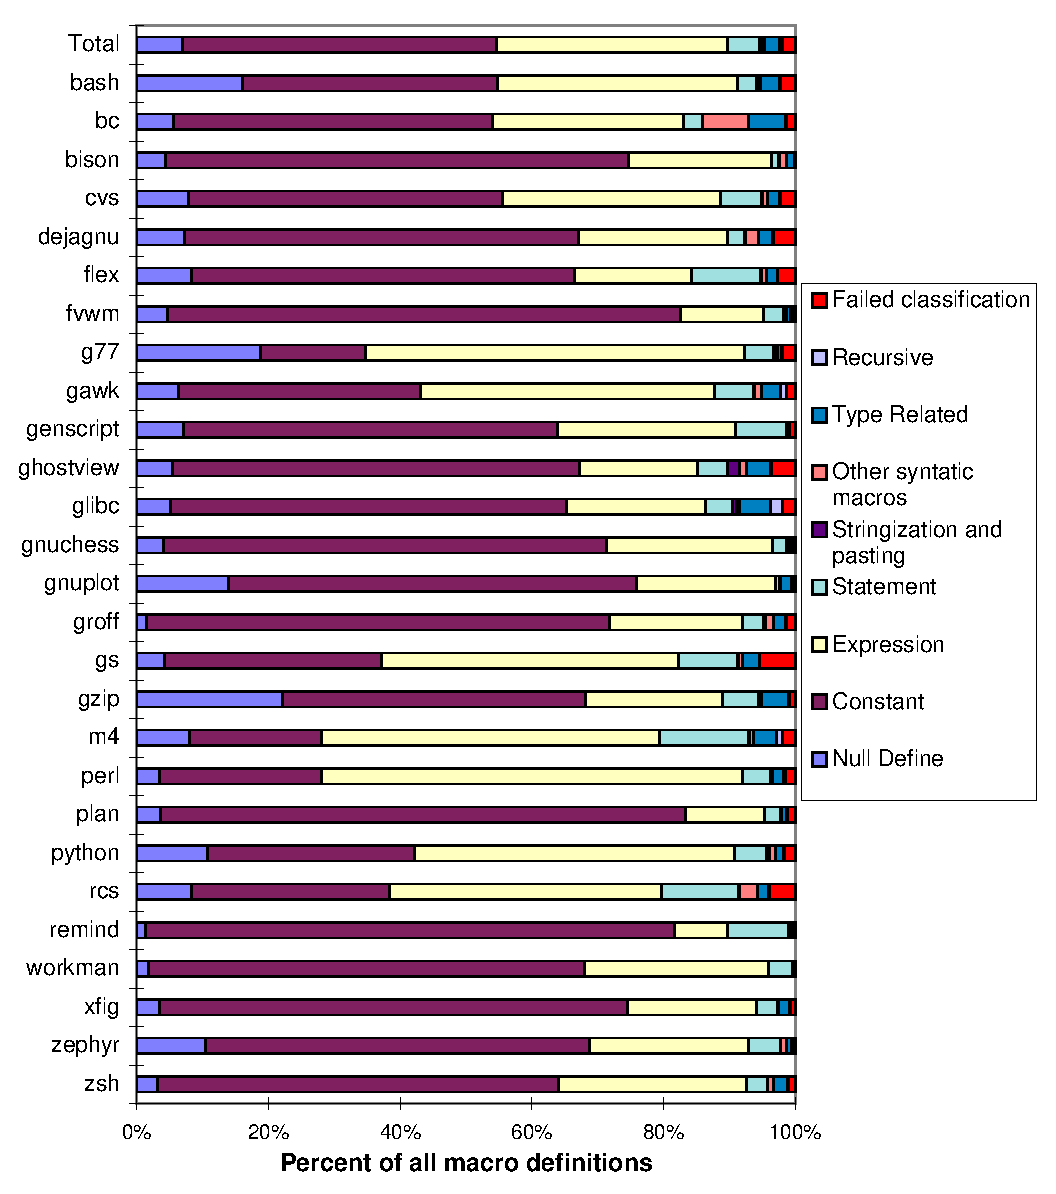
\epsfig{file=def-categories.eps,height=\epsheight}}

Less than 3\% of macros have incompatible multiple definitions
\end{slide}

\begin{note}
Good news and bad: \slbreak
most are simple:  simple for me to cope with, simple for other tools as
well (so no need for someone clever to worry about all this) \slbreak
There are few bad ones percentagewise, but many numerically, and they are
the tough ones, after all.

Most common ``conflict,'' between statement and null define (0.42\%), is
usually harmless
\end{note}


\begin{slide}
\slidetitle{Improving C/Cpp}

Translate into {\tt const}, {\tt inline}, templates, reference parameters,
{\tt bool}, {\tt enum}, \ldots

Standardize library interfaces

Single, more flexible declaration syntax

Language support for Cpp tasks

Don't make Cpp more powerful!
\end{slide}

\begin{note}
This is really about improving {\em understandability}

Libraries: standardize function names, calling conventions.  This moves the
responsibility from application programmer to library/systems programmer. 

Language support: {\tt \#include}, (partial) declarations

Making Cpp more powerful is attractive theoretically, but a disaster for
software engineers: doesn't lead to more understanable programs.
\end{note}


\begin{slide}
\slidetitle{Future work}

Parse more C:  typedefs, structs, precedence

Macro lint:
\vspace{-.5in}
\begin{itemize}\itemsep 0pt \parskip 0pt
\item side effects
\item semicolon swallowing
\item free variables
\item more...
\end{itemize}

Infer types

Translate

Partially specify macro values

Transitive dependences

Macro dependence structure/lattice

\end{slide}

\begin{note}
\small
Perhaps this is the time to discuss the tool (not a very interesting
topic).

Side effects: if actual has side effect and formal used multiple times; if
body has side effect, can't be a const (but can be turned into a formal, and
maybe the compiler will be able to figure something out)

Infer types:
 can't know real types without knowledge of architecture
 the type of zero
 polymorphism

Translation:
 macros can go where functions can't, like case labels
 the enum hack
 idiomatic C++, e.g. use of bool, enum.  (Just a tool that introduced bool
     would be quite nice...)

Polymorphism:
2 cases where macros provide polymorphism:
 * type argument
 * use of ad-hoc polymorphism inherited from underlying operators, e.g.
     min works on both floats \& ints, or both shorts \& longs (the latter
     can't be converted to long w/o loss of efficiency)
Can't capture this without templates -- can't even tell when it is
really being used, though could avoid doing some type promotion (say,
beyond int or unsigned int).
Macros too relaxed, too polymorphic (e.g. can pass char to ABS macro, but
that wasn't intended; on the other hand, same thing happens for a function,
right?).  The translation will indicate this.  Do we want a
template or just specific types?
Making every macro into a template function works well, because the calls
don't change, just the definitions.  (But declarations in the body might
change, so it involves parsing and rewriting the body, not just the
declaration.  And, what is the return type?)
\end{note}


\end{document}
